\newpage
\section{Preventivo Iniziale}

\begin{figure}[H]
\begin{center}
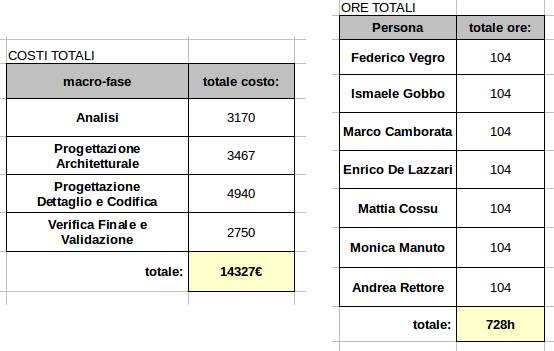
\includegraphics[scale=0.50]{img/totali.png}
\caption{Tabelle dei costi e delle ore totali.}
\end{center}
\end{figure}

Dalla sezione \ref{pianificazione} si ricava un costo totale del progetto di \textbf{14327€}, e 104 ore complessive di lavoro per ciascun membro del gruppo.

\section{Consuntivi e Preventivi a finire}
In questa sezione viene riportato il prospetto economico di ogni macro-fase conclusa, che evidenzia la differenza tra le spese previste e quelle effettivamente sostenute.

\subsection{Progettazione Architetturale}
\subsubsection{Consuntivo parziale}
Nella stesura iniziale del piano è stato largamente sottovalutato il tempo necessario per acquisire le conoscenze atte a chiarire come saranno strutturati i componenti e le classi del prodotto. Questo ha portato a non rispettare le date di consegna per la prima Revisione di Progettazione, e a spostare tutte le successive consegne alla prossima data disponibile. \\
Si è cercato nel migliore dei modi di chiarire quale parte di questo studio fosse rivolta all'apprendimento delle tecnologie adottate, e quindi a carico del gruppo, e quale invece riguardasse la creazione di una visione di insieme dei componenti di Premi, parte cruciale nella stesura della Specifica Tecnica: ne è risultata una diminuzione delle ore di lavoro dei progettisti, che si sono potuti dedicare alla stesura di altre parti del documento. \\
L'esito della Revisione dei Requisiti ha portato ad uno studio non previsto di nuove funzionalità, con un inevitabile aumento delle ore di lavoro dedicate alla correzione dell'Analisi dei Requisiti. \\
Le rimanenti attività si sono susseguite rispettando i tempi prestabiliti; la tabella seguente mostra in verde le ore risparmiate e in rosso quelle non previste. \\

\begin{figure}[H]
\begin{center}
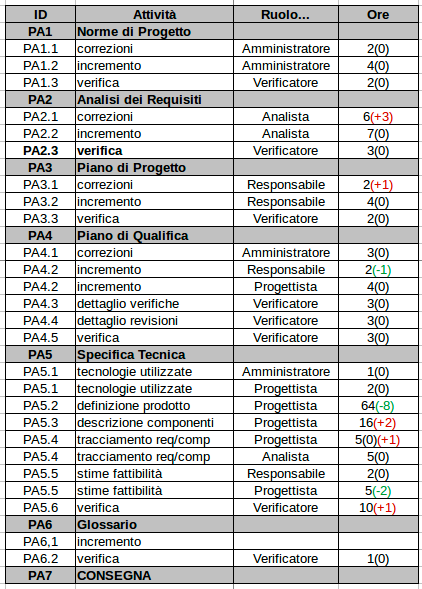
\includegraphics[scale=0.65]{img/consuntivo-progarc.png}
\caption{Tabella delle ore previste e sostenute nella Progettazione Architetturale.}
\end{center}
\end{figure}

Dalla tabella precedente risulta una differenza di soli \textbf{2€} in questa macro-fase rispetto a quanto preventivato. \\

\begin{figure}[H]
\begin{center}
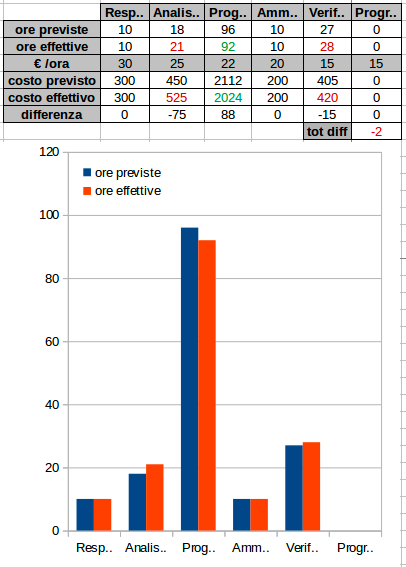
\includegraphics[scale=0.70]{img/consuntivo-progarc-tot.png}
\caption{Tabella dei costi totali previsti e sostenuti nella Progettazione Architetturale.}
\end{center}
\end{figure}

\subsubsection{Preventivo a Finire}
 Lo studio delle tecnologie effettuato da tutti i membri del gruppo dovrebbe portare ad un risparmio di tempo nella prossima macro-fase, ma rimangono ancora da effettuare ulteriori approfondimenti sull'utilizzo di alcune librerie esterne. Le ore di lavoro impiegate finora non si discostano da quelle stimate,  pertanto in questa macro-fase non verranno ancora apportate modifiche al preventivo iniziale.


\subsection{Progettazione di Dettaglio e Codifica}

\subsubsection{Consuntivo parziale}
Le ore effettive di questa macro-fase sono state molto diverse rispetto a quelle inizialmente preventivate nella fase di Analisi. Oltre alle correzioni aggiuntive, già previste in precedenza, sull'architettura di Premi, le ore di codifica dedicate dai programmatori alla risoluzione di problemi relativi alle librerie esterne scelte per il progetto hanno portato un aumento considerevole del tempo dedicato al progetto da parte del gruppo, con conseguenti ritardi sulla tabella di marcia. Per queste ragioni alcuni dei requisiti opzionali o desiderabili non sono ancora completamente soddisfatti dall'applicazione, e alcune parti dell'editor appaiono ancora troppo meccaniche e rudimentali; il Manuale Utente inoltre non è ancora ad un stato sufficientemente maturo per definire con precisione le funzionalità dell'applicazione. \\ 
Ritardi aggiuntivi sono stati inoltre causati da cambiamenti sull'utilizzo di jQuery$_G$ che era stato erroneamente utilizzato al posto di funzionalità del framework AngularJS$_G$, e dalle vacanze estive non sempre comunicate per tempo in modo da garantire una suddivisione delle ore efficace.
Sfruttando il programma Velocity$_G$ e il componente esterno Jasmine$_G$ per la codifica dei test di unità si è riscontrato invece un risparmio di tempo dovuto all'automazione di molti dei controlli sui metodi scritti finora. 


\begin{figure}[H]
\begin{center}
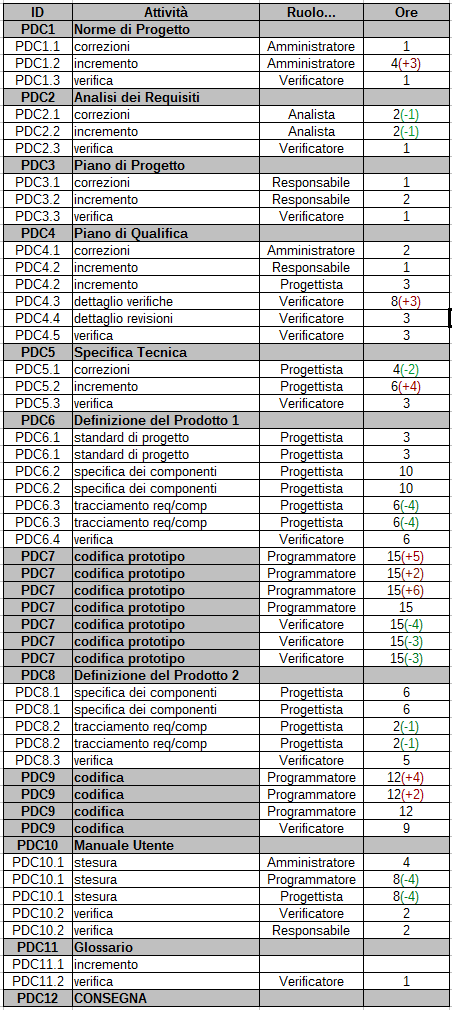
\includegraphics[scale=0.75]{img/consuntivo-progdet.png}
\caption{Tabella delle ore previste e sostenute nella Progettazione di Dettaglio e Codifica.}
\end{center}
\end{figure}

Dalla tabella precedente risulta un aumento dei costi di produzione di \textbf{134€} in questa macro-fase rispetto a quanto preventivato, causato dall'aumento delle ore dedicate alla codifica del prodotto.

\begin{figure}[H]
\begin{center}
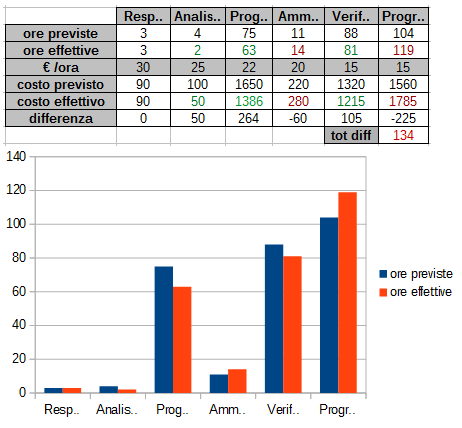
\includegraphics[scale=0.70]{img/consuntivo-progdet-tot.png}
\caption{Tabella delle ore previste e sostenute nella Progettazione di Dettaglio e Codifica.}
\end{center}
\end{figure}

\subsubsection{Preventivo a Finire}
L'applicazione non è ancora completa e sono previsti degli incrementi nella maggior parte dei suoi componenti. Questo comporterà ulteriori ore di lavoro non preventivate che saranno svolte gratuitamente dal gruppo. Le cause di questi ritardi derivano dall'inesperienza del gruppo ad affrontare problemi di compatibilità tra le tecnologie adottate e le librerie esterne indispensabili al funzionamento di alcune parti del prodotto. \\
Essendo rimasta una sola convocazione disponibile, ed essendo rimasto ormai poco tempo disponibile si prevede che alcuni requisiti opzionali andranno trascurati, per dedicare maggiore attenzione alle funzionalità obbligatorie previste nella fase di Analisi. \\
Il carico di lavoro verrà distribuito il più equamente possibile e i rischi definiti in questo documento verranno controllati giornalmente tramite un controllo continuo dei ticket assegnati.




